\subsection{Neural Networks}
\label{sec::321_nn}
\cite{weng1992cresceptron} % max pooling
\cite{krizhevsky2012imagenet} % relu
\subsubsection{Fully Connected Neural Network}
%
\begin{figure}[h]
	\centering
	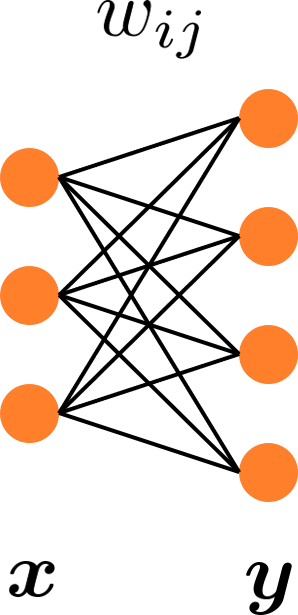
\includegraphics[scale=.28]{chapters/03_background/img/fully_connected.png}
	\caption{Fully connected neural network with three inputs and four outputs. Each orange circle represents what is often referred to as neuron, while the black lines indicate the connections between each neuron.}
	\label{fig::321_fully_connected}
\end{figure}
\subsubsection{Convolutional Neural Network}
\cite{fukushima1980neocognitron} % convolutional neural networks under neocognitron
\begin{figure}[h]
	\centering
	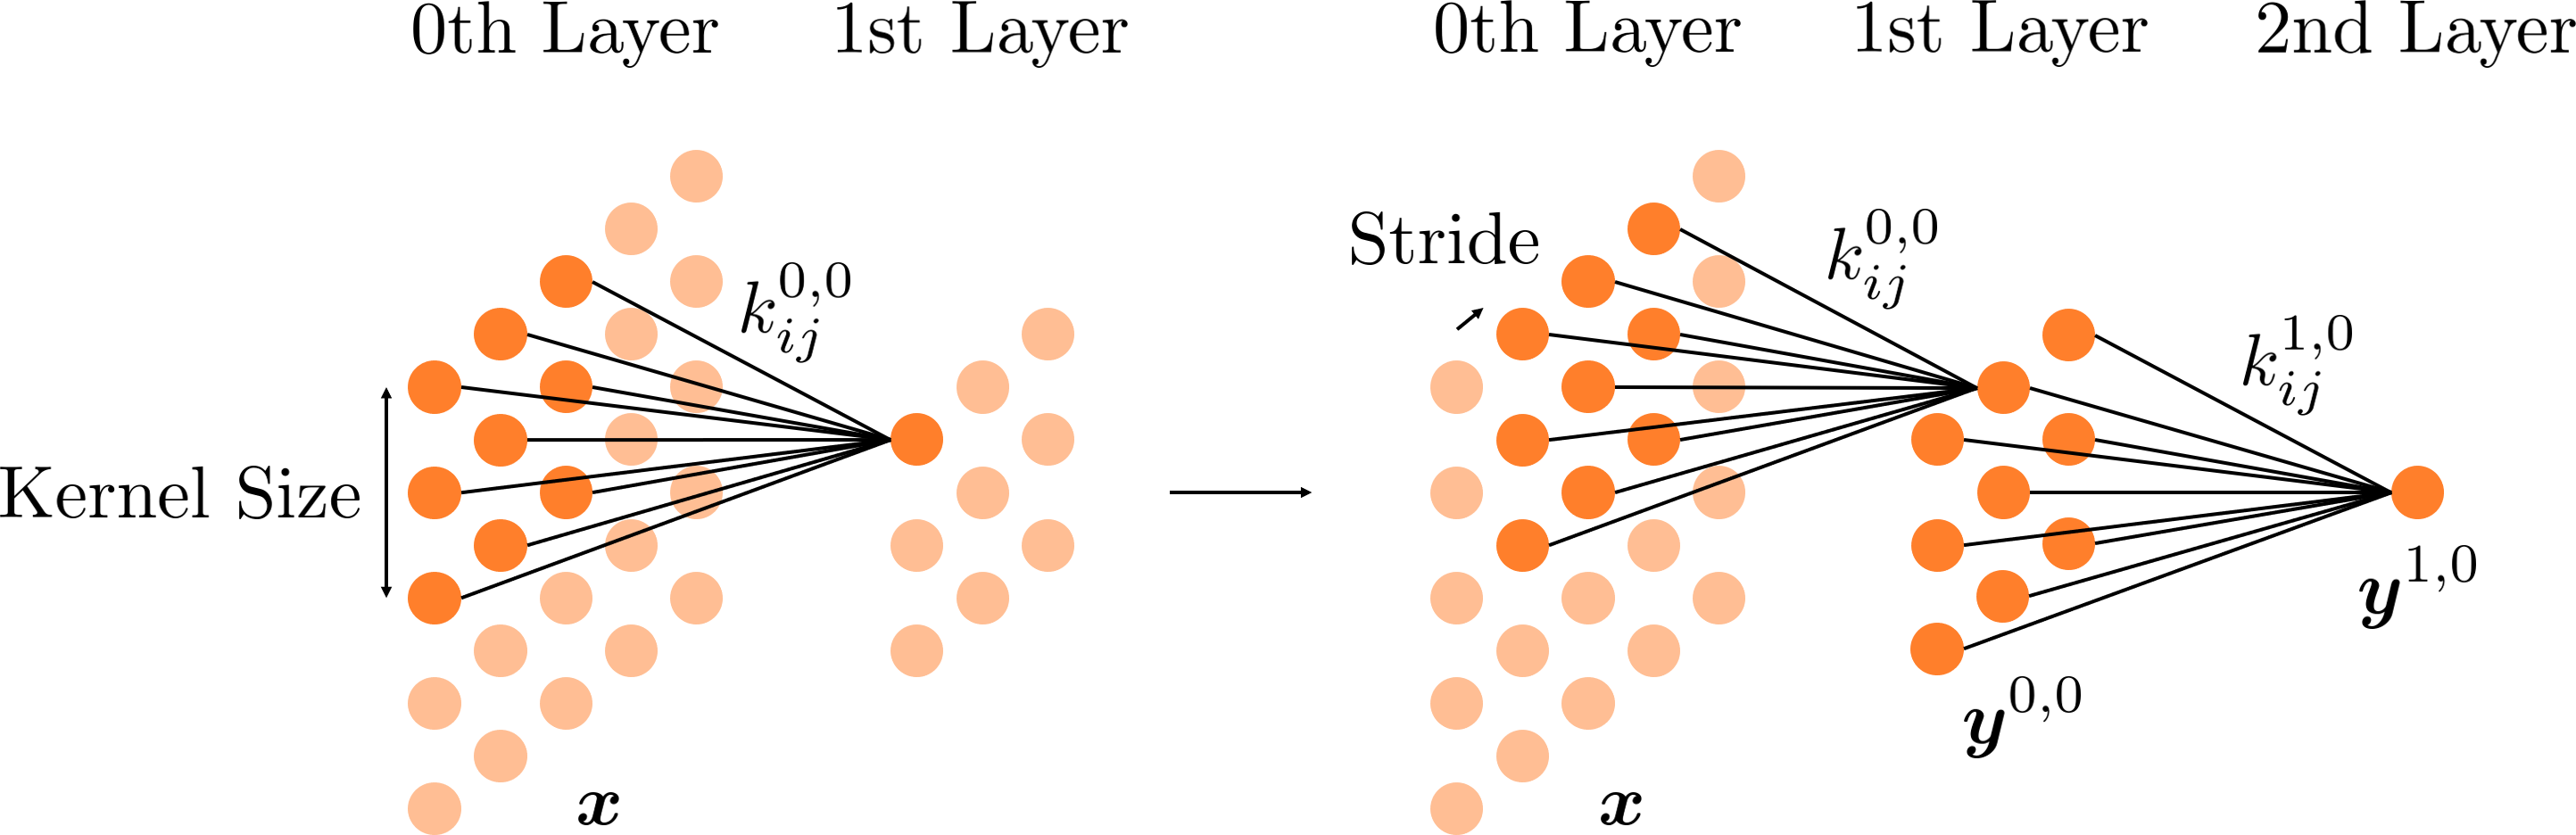
\includegraphics[scale=.28]{chapters/03_background/img/convolutional.png}
	\caption{Convolutional neural network with a total of three layers of which one is the input layer. For visualization, the kernel size is set to be three, and the stride is set to be one.}
	\label{fig::321_convolutional}
\end{figure}
\subsubsection{Long Short-Term Memory}
\cite{hochreiter1997long} % lstm
\begin{figure}[h]
	\centering
	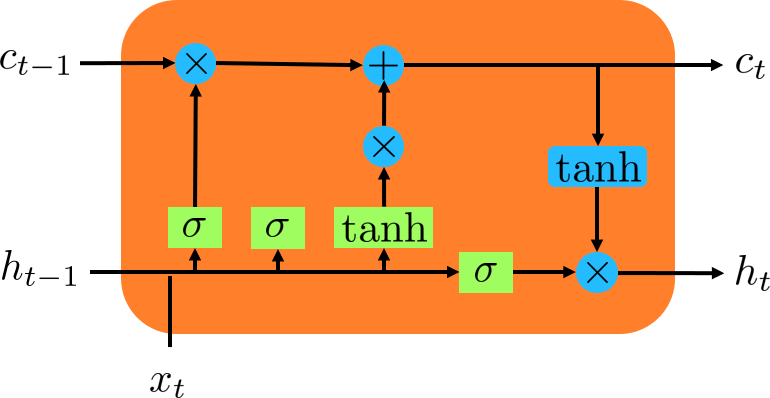
\includegraphics[scale=.28]{chapters/03_background/img/lstm.png}
	\caption{Long short-term memory unit with cell states $\bm{c}_i$, hidden states $\bm{h}_i$, input $\bm{x}_t$, and activation functions $\sigma/\tanh$, as well as addition $+$ and multiplication $\times$ operators.}
	\label{fig::321_lstm}
\end{figure}
\begin{figure}[h]
	\centering
	
\includegraphics[scale=.28]{chapters/03_background/img/lstm_chain.png}
	\caption{Chain of long short-term memory units for temporal understanding of the input sequence $\bm{x}_i$.}
	\label{fig::321_lstm_chain}
\end{figure}
\subsubsection{Backpropagation}
\cite{linnainmaa1970representation}